\documentclass{article}
\usepackage{amsmath}
\usepackage{tikz}
\usepackage{xparse}
%% LOCAL style file — collect_macros must resolve and read it
\usepackage{authorstyle}

%% --- six macro definitions, in six different forms ------------------------
\newcommand{\newcmdMacro}[1]{\mathrm{#1}}          % 1  handled
\def\defMacro#1{\mathit{#1}}                        % 2  handled
\DeclareMathOperator{\opMacro}{opm}                 % 3  handled
%% 4 is \styleMacro, defined in authorstyle.sty
\NewDocumentCommand{\xparseMacro}{m}{\mathbb{#1}}   % 5  xparse
\let\letMacro\newcmdMacro                           % 6  \let

%% a custom environment, which is not a macro and not a graphic env
\newenvironment{authorbox}{\begin{center}}{\end{center}}

\begin{document}

%% --- three graphic forms --------------------------------------------------
% (a) the environment form
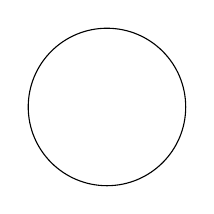
\begin{tikzpicture}
  \draw (0,0) circle (1);
\end{tikzpicture}

% (b) inline, braced:  \tikz[opts]{...}
\tikz[baseline]{\draw (0,0) -- (1,0);}

% (c) inline, semicolon-terminated:  \tikz ... ;
\tikz \draw (0,0) -- (0,1);

\begin{authorbox}
  Text inside the author's own environment.
\end{authorbox}

%% the thesis construct: a margin note with an offset, holding a picture.
%% Brace-matched or the closing } of the tikzpicture ends the note early.
\marginnote[-6cm]{A note, with \begin{tikzpicture}\draw (0,0) -- (2,2);\end{tikzpicture} inside.}

%% a tikzpicture reached only through \input
%% \input'ed body. The tikzpicture here is only visible to extract_graphics
%% if the caller inlined the \input first -- build_source_model does, a
%% direct call does not.
\begin{tikzpicture}
  \draw (0,0) -- (1,1);
\end{tikzpicture}


Uses: \newcmdMacro{a} \defMacro{b} \opMacro \styleMacro{d}
      \xparseMacro{e} \letMacro{f}

\end{document}
